%%%%%%%%%%%%%%%%%%%%%%%%%%%%%%%%%%%%%%%%%
% Sullivan Business Report
% LaTeX Template
% Version 1.0 (May 5, 2022)
%
% This template originates from:
% https://www.LaTeXTemplates.com
%
% Author:
% Vel (vel@latextemplates.com)
%
% License:
% CC BY-NC-SA 4.0 (https://creativecommons.org/licenses/by-nc-sa/4.0/)
%
%%%%%%%%%%%%%%%%%%%%%%%%%%%%%%%%%%%%%%%%%

%----------------------------------------------------------------------------------------
%	CLASS, PACKAGES AND OTHER DOCUMENT CONFIGURATIONS
%----------------------------------------------------------------------------------------

\documentclass[
	a4paper, % Paper size, use either a4paper or letterpaper
	12pt, % Default font size, the template is designed to look good at 12pt so it's best not to change this
	%unnumberedsections, % Uncomment for no section numbering
]{CSSullivanBusinessReport}

\addbibresource{references.bib} % BibLaTeX bibliography file


% \usepackage{background} 
% \backgroundsetup{contents=DRAFT-2} % Set your own text 

%----------------------------------------------------------------------------------------
%	REPORT INFORMATION
%----------------------------------------------------------------------------------------

\reporttitle{POKT AI Lab} % The report title to appear on the title page and page headers, do not create manual new lines here as this will carry over to page headers

\reportsubtitle{Report III} % Report subtitle, include new lines if needed

\reportauthors{Authors:\\\smallskip  Nicolas Aguirre (nicolas@poktscan.com)\\ Ramiro Rodr\'iguez Colmeiro (ramiro@poktscan.com)\\ POKTscan Data Science Team }

\reportdate{\today} % Report date, include new lines for additional information if needed

\rightheadercontent{
\includegraphics[width=3cm]{POKT_logo.png}} % The content in the right header, you may want to add your own company logo or use your company/department name or leave this command empty for no right header content

%----------------------------------------------------------------------------------------

%\usepackage[printwatermark]{xwatermark}
%\newwatermark[allpages,color=red!30,angle=45,scale=6,xpos=-2cm,ypos=0]{DRAFT}  

\usepackage{placeins}

%%%%%%%%%%%%%%%%%%%%%%%%%
% Subplots
%%%%%%%%%%%%%%%%%%%%%%%%%
%\usepackage{subcaption}
%\usepackage[labelformat=simple]{subcaption} %Para subplots con parentesis
%\renewcommand\thesubfigure{(\alph{subfigure})}


\usepackage{amsmath,amssymb,amsfonts,amsbsy,latexsym,mathtools,bm}%,bbm} 

\usepackage[acronym,toc,nomain,nonumberlist,nogroupskip]{glossaries-extra}
\setglossarystyle{alttree} %Description tabulation
\glssetwidest{Holistic Evaluation of Language Models} % Longest acronym
\makeglossaries
\loadglsentries{acronym_def} % file.tex

%%%%%%%%%%%%%%%%%%%%%%%%%
% Espacio entre palabras: \usepackage{setspace}
%%%%%%%%%%%%%%%%%%%%%%%%%
\usepackage{setspace}
\onehalfspacing
%%%%%%%%%%%%%%%%%%%%%%%%%
% Para fracciones con slash
%%%%%%%%%%%%%%%%%%%%%%%%%
\usepackage{nicefrac, xfrac}

%Texbox
\usepackage{tcolorbox}
\usepackage{lipsum}

% Quotes
\usepackage{epigraph} 

\begin{document}

%----------------------------------------------------------------------------------------
%	TITLE PAGE
%----------------------------------------------------------------------------------------

\thispagestyle{empty} % Suppress headers and footers on this page

%\begin{fullwidth} % Use the whole page width
	\vspace*{-0.075\textheight} % Pull POKT latex template logo into the top margin
	
	\hfill
\includegraphics[width=5cm]{POKT_logo.png} % Company logo

	\vspace{0.15\textheight} % Vertical whitespace

	\parbox{0.9\textwidth}{\fontsize{50pt}{52pt}\selectfont\raggedright\textbf{\reporttitle}\par} % Report title, intentionally at less than full width for nice wrapping. Adjust the width of the \parbox and the font size as needed for your title to look good.
	
	\vspace{0.03\textheight} % Vertical whitespace
	
	{\LARGE\textit{\textbf{\reportsubtitle}}\par} % Subtitle
	
	\vfill % Vertical whitespace
	
	{\Large\reportauthors\par} % Report authors, group or department
	
	\vfill\vfill\vfill % Vertical whitespace
	
	{\large\reportdate\par} % Report date
%\end{fullwidth}

\newpage

%----------------------------------------------------------------------------------------
%	DISCLAIMER/COPYRIGHT PAGE
%----------------------------------------------------------------------------------------

\thispagestyle{empty} % Suppress headers and footers on this page

%\begin{twothirdswidth} % Content in this environment to be at two-thirds of the whole page width
	\footnotesize % Reduce font size
	
	\subsection*{Disclaimer}
	
	This work was partially funded by Pocket Scan Technologies LLC, a company operating on the Pocket Network.

	\vfill % Push the following down to the bottom of the page
	
	\subsubsection*{Changelog}
	
	\scriptsize % Reduce font size further
	
	\begin{tabular}{@{} L{0.05\linewidth} L{0.15\linewidth} L{0.6\linewidth} @{}} % Column widths specified here, change as needed for your content
		\toprule
		v1.0 & 2024-05-30 & First version.\\
		\bottomrule
	\end{tabular}
%\end{twothirdswidth}

\normalsize
\newpage

%----------------------------------------------------------------------------------------
%	TABLE OF CONTENTS
%----------------------------------------------------------------------------------------

%\begin{twothirdswidth} % Content in this environment to be at two-thirds of the whole page width
    \doublespacing
    \tableofcontents % Output the table of contents, automatically generated from the section commands used in the document
    \onehalfspacing
%\end{twothirdswidth}

\newpage

%----------------------------------------------------------------------------------------
%	SECTIONS
%----------------------------------------------------------------------------------------
\section{Progress Overview}\label{sec:a}

During the month of June, the socket achieved the following milestones:

\begin{itemize}[noitemsep]
    \item Merged issues on the Test-Bench code:
    \begin{itemize}[noitemsep]
        \item \textbf{Manager}:
            \begin{itemize}[noitemsep]
                \item Add same trigger restrictions based on blocks. \footnote{\url{https://github.com/pokt-scan/pocket-ml-testbench/pull/67}}
                \item Create logic for tokenizer signature task. \footnote{\url{https://github.com/pokt-scan/pocket-ml-testbench/pull/62}}
            \end{itemize}
        \item \textbf{Sampler}:
            \begin{itemize}[noitemsep]
                \item Create logic for tokenizer signature task. \footnote{\url{https://github.com/pokt-scan/pocket-ml-testbench/pull/57}}
                \item Fix generation\_until in LM classes. \footnote{\url{https://github.com/pokt-scan/pocket-ml-testbench/pull/78}}
            \end{itemize}
        \item \textbf{Evaluator}:
            \begin{itemize}[noitemsep]
                \item Create initial code for lmeh processing. \footnote{\url{https://github.com/pokt-scan/pocket-ml-testbench/pull/60}}
                \item Add signatures tokenizer evaluation. \footnote{\url{https://github.com/pokt-scan/pocket-ml-testbench/pull/63}}
                \item Finish code for lmeh. \footnote{\url{https://github.com/pokt-scan/pocket-ml-testbench/pull/65}}
            \end{itemize}
        \item \textbf{Sidecard}:
            \begin{itemize}[noitemsep]
                \item Added endpoint for tokenizer in llm nodes. \footnote{\url{https://github.com/pokt-scan/pocket-ml-testbench/pull/56}}                
            \end{itemize}
        \item \textbf{General}:
            \begin{itemize}[noitemsep]
                \item Modularizing the tasks to allow signatures. \footnote{\url{https://github.com/pokt-scan/pocket-ml-testbench/pull/54}}
                \item Task configs: update metrics and filters. \footnote{\url{https://github.com/pokt-scan/pocket-ml-testbench/pull/80}}
                \item Added website to show metrics. \footnote{\url{https://github.com/pokt-scan/pocket-ml-testbench/pull/81}}
                \item Full ML Test bench integration. \footnote{\url{https://github.com/pokt-scan/pocket-ml-testbench/pull/83}}            
            \end{itemize}
    \end{itemize}
\end{itemize}

In June 2024, significant progress was made on the socket, culminating in the completion of various tasks and milestones. 
Finally the different components of the \gls{MLTB}, such as the Manager, Sampler, Evaluator, and Sidecard were integrated. 
This integration culminated presenting the leaderboards on a website considering the results of the corresponding task metrics.

In the next sections of the present report the details of these developments and their implications are presented. 
These sections provide an overview of the work completed, updating components initially considered, and the progress made towards the final goal of the socket.

Furthermore, looking ahead, there are several future work ideas to consider. 
These include refining the evaluation metrics further, exploring additional benchmark for extended functionalities. 
These future initiatives aim to enhance the network capacity guided by the state-of-the-art in the field of machine learning and blockchain technology.


\begin{tcolorbox}[colback=red!5!white,colframe=red!75!black]
\textbf{Note:} This report was written \today, and the Huggingface announced an update in the \gls{HFOLML} at Jun 26, 2024. 
In comparison to the socket scope, major change are related to unimplemented tasks, new metrics, and task higly related to chat models. 
On the other hand, there are tasks that just have new configs. 
This report will not cover the new Leaderboard. 
Nevertheles, at POKTscan and PNYX, we are confident that the \gls{MLTB} is ready to be developed in order to reproduce the \textbf{old} Leaderboard. 
furthermore, we except that the \gls{MLTB} will be able in a short time to be updated to the new Leaderboard. 

Addressing evaluations of \gls{LM}, a topic that is at the forefront of knowledge, has an inherently dynamic nature. 
That is to say, the constant (and increasingly accelerated) improvement of the \gls{LM} requires the development of new evaluations that have to be constantly improved. 
What happened with the \gls{HFOLML} is just the first case Pocket Network faces when it wants to support AI in it. 
At POKTscan we alert the community about this inevitable game of cat and mouse, and we encourage everyone to join the game. 
\end{tcolorbox}
\section{Language Models - Tokenizer}\label{sec:b}

In this sections is briefly introduced the concept of \textit{token}, \textit{tokenization} and \textit{tokenizer}, how it works in a \gls{LM}, an issue when running a decentralized benchmarking, and finally a proposed solution. 

\subsection{From string to token}\label{subsec:b1}

Tokenization is the process of representing text in smaller meaningful lexical units. 
There are three popular ways to do the same, which are: 1) word tokenization, 2) subword tokenization, and 3) character tokenization. 
Word tokenization is the simplest form of tokenization, where each word is considered a token. 
Subword tokenization breaks words into subwords and treats them as tokens. 
Character tokenization considers each character as a token. 
There is a trade-off between the granularity of the tokens and the number of tokens. 
That is, while word tokenization has low granularity and high token count, character tokenization has high granularity and low token count. 
Nowadays, the most popular tokenization method is subword tokenization, which is a compromise between word and character tokenization.
It is important to note that prior to training a model, tokenizers must be trained on texts that is representative of the training set (ideally the tokenizer texts should not be part of the training set). 
With respect to the tokenizer trainin method it's worth to mention that there exist several techniques \cite{kudo_sentencepiece_2018,kudo_subword_2018,sennrich_neural_2016}

On the other hand, the tokenizer is the one in charge of carrying out the tokenization process, which consists (in a nutshell) of a dictionary that contains pairs of tokens and their numerical representation. 
For this reason, a direct relationship is established between a \gls{LM} and its tokenizer, which is crucial when evaluating the performance of a \gls{LM} since one of the main techniques for evaluating a language \gls{LM} is through the calculation of the probability of occurrence of a sequence of tokens that is conditioned by an initial sequence of tokens. 
In terms of \texttt{lm-eval-harness}\cite{biderman_lessons_2024} these two sequences are also called \texttt{context} and \texttt{continuation}, as shown in Figure \ref{fig:loglikelihood_example}.

\begin{figure}[h]
    \centering
    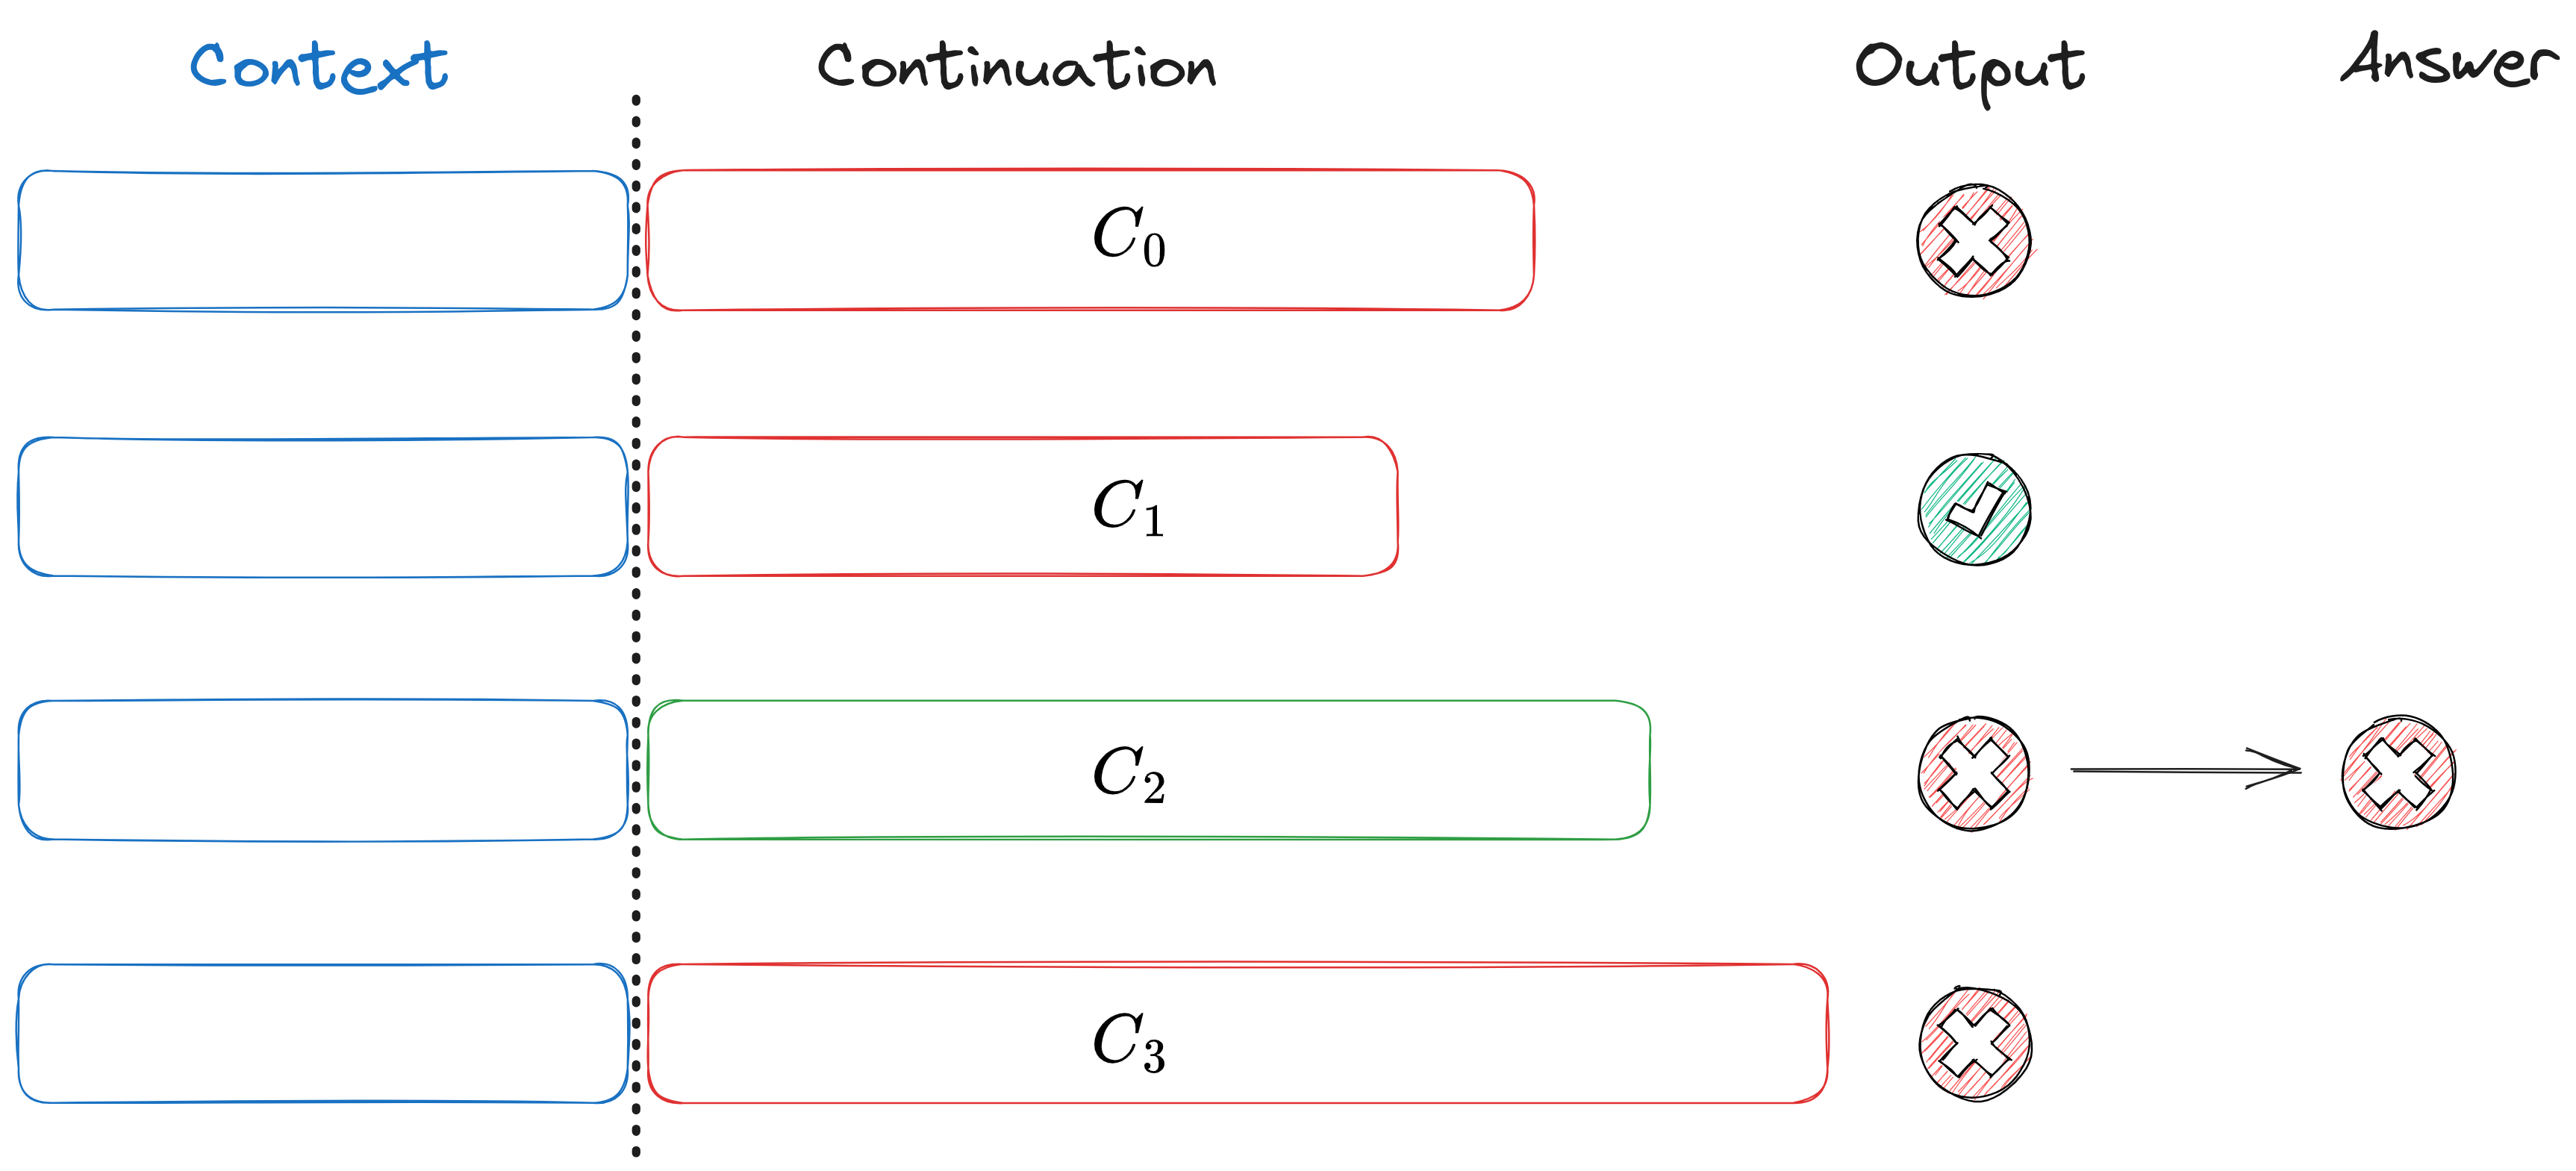
\includegraphics[width=0.8\textwidth]{img/loglikelihood_example.png}
    \caption{Example of \texttt{context} and \texttt{continuation} token sequences.}
    \label{fig:loglikelihood_example}
\end{figure}

Without going into the mathematical details, and following the Figure \ref{fig:loglikelihood_example}, the concatenation of the \texttt{context} and \texttt{continuation} tokens is sent to the language models, and from the \gls{LM} returns it can be computed the probability of occurrence of the entire phrase detailed token by token. 
The \gls{LM} is considered to respond correctly when the probability of occurrence of the correct \texttt{continuation} is the highest with respect to the other continuations. That is, in terms of the Figure \ref{fig:loglikelihood_example}, the \gls{LM} responds incorrectly, since $C_2$ should have been the \texttt{continuation} with the highest probability, but the \gls{LM} returns a higher probability for $C_1$. 

\subsection{On the lack of knowledge of the tokenizer}\label{subsec:b2}

As previously detailed, the \gls{LM} receives the concatenation of the \texttt{context} and \texttt{continuation} token sequences, and then locally separates the \texttt{context} and \texttt{continuation} probabilities. 
However, in a decentralized environment, such as that proposed by benchmarking, if you do not have access to the tokenizer, it is not possible to separate the \texttt{context} and \texttt{continuation} probabilities. 
The plain text of the concatenation of contex and \texttt{continuation} could be sent, but then we could not directly determine which part of the text belongs to the \texttt{context} and which part belongs to the continuation, thus preventing the evaluation of the model. 
Although one could try to reconstruct the \texttt{context} and \texttt{continuation} phrase from the concatenation of tokens, this is not a trivial task, since the tokenizer could have tokenized differently than the original text was tokenized \cite{biderman_lessons_2024}. 

\subsection{Proposed solution}\label{subsec:b3}

Faced with this situation, there are three other plausible solutions. 
The first solution would be to send, in addition to each complete sentence, only the \texttt{context} text. 
This would then allow us to remove those corresponding to the \texttt{context} from each of the complete sentences and continue with the evaluation of the model. 
The disadvantage of this solution is that $N+1$ calls would be made to the model, where $N$ is the number of complete sentences to evaluate, resulting in a higher cost. 
Furthermore, in the case of evaluations that contemplate the use of conversational models (such as the case of chat), this solution would not be applicable, since internally these models through its toke add special tokens to indicate the beginning and end of a message in a conversation, just as they usually have a text to condition the model's response, called system prompt. 
The second solution would be online tokenization, calling for example an endpoint \emph{tokenize}. 
This situation would face similar problems, as currently discussed in the community \footnote{\url{https://github.com/huggingface/text-generation-inference/issues/1706}}. 
The third solution would involve sending the complet tokenizer associated with an node address. 
This was detailed in two PRs \footnote{\url{https://github.com/EleutherAI/lm-evaluation-harness/pull/1794}} \footnote{\url{https://github.com/vllm-project/vllm/pull/2643}} in both the lm-eval-harness repository and the vLLM repository, popular \gls{LM} inference engine. 
The main advantage of this solution is that the issues of the first and second solutions are avoided. 
Additionally, as previously detailed, the tokenizer is tied to the model. 
Therefore we can generate a hash of the tokenizer that sends us an address, save it in a database and then verify that the hash of the tokenizer that is sent at the beginning of a session is equal to the hash stored in the database. 
If for some reason the hash does not match, it is an unequivocal indication that the \gls{LM} behind the endpoint is not the same, it has changed, therefore the previous results are not valid, metrics are eliminated from the leaderboard, and that address has to be re-evaluated. 
\section{Future Work}\label{sec:z}

hablar de que pokt-square no lo vamos a seguir laburando activamente.

decir cuales son las cosas que siguen en desarrollo

dar panorama para cuando primer mvp?
\newpage


%----------------------------------------------------------------------------------------
%	 Acronyms
%----------------------------------------------------------------------------------------
\printglossary[type=\acronymtype,title=List of Acronyms]

%----------------------------------------------------------------------------------------
%	 REFERENCES/BIBLIOGRAPHY
%----------------------------------------------------------------------------------------

\newpage

\addcontentsline{toc}{section}{Reference List} % Add the bibliography to the table of contents

%\begin{twothirdswidth} % Content in this environment to be at two-thirds of the whole page width
	\printbibliography[title=Reference List] % Output the bibliography with a custom section title
%\end{twothirdswidth}


%----------------------------------------------------------------------------------------

\end{document}	


